\chapter{Architecture Diagram and Conceptual Model}

\section{Architecture}
The system relies on an event-based architecture. As shown in the architecture diagram (Figure \ref{fig:architecture}), the arrows show the flow of data between the different components of the system. The doorbell button triggers an event that goes to the Raspberry Pi Zero which acts as an announcer in this architecture. This event tells the announcer to broadcast the appropriate doorbell event to all types of devices currently registered in the system. The doorbell offers feedback to the Visitor in the form of a pulsating light to confirm that the button was pressed and the event was broadcast to the Resident's devices. The arrow going to the Raspberry Pi Zero from the Home Network is to confirm that the devices received the broadcast event.

\begin{figure}[ht]
  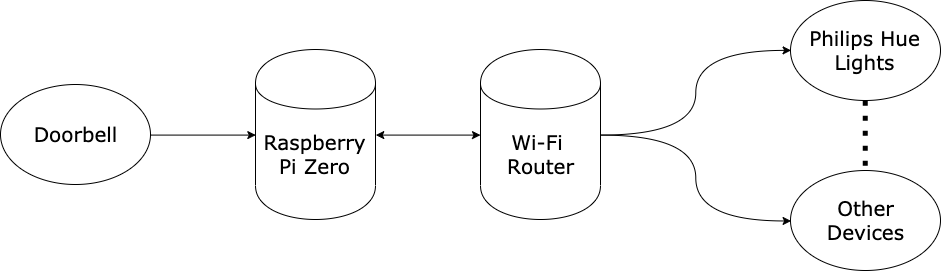
\includegraphics[width=0.9\textwidth]{Architecture-updated.png}
  \centering
  \caption{Architecture Diagram}
  \label{fig:architecture}
\end{figure}

\section{Conceptual Model}
The system uses the Raspberry Pi Zero as the main gateway. A router will be necessary in communicating to other devices in the household. The button of the doorbell will be attached to the an Arduino and communicate with the Raspberry Pi Zero.

\begin{figure}[ht]
  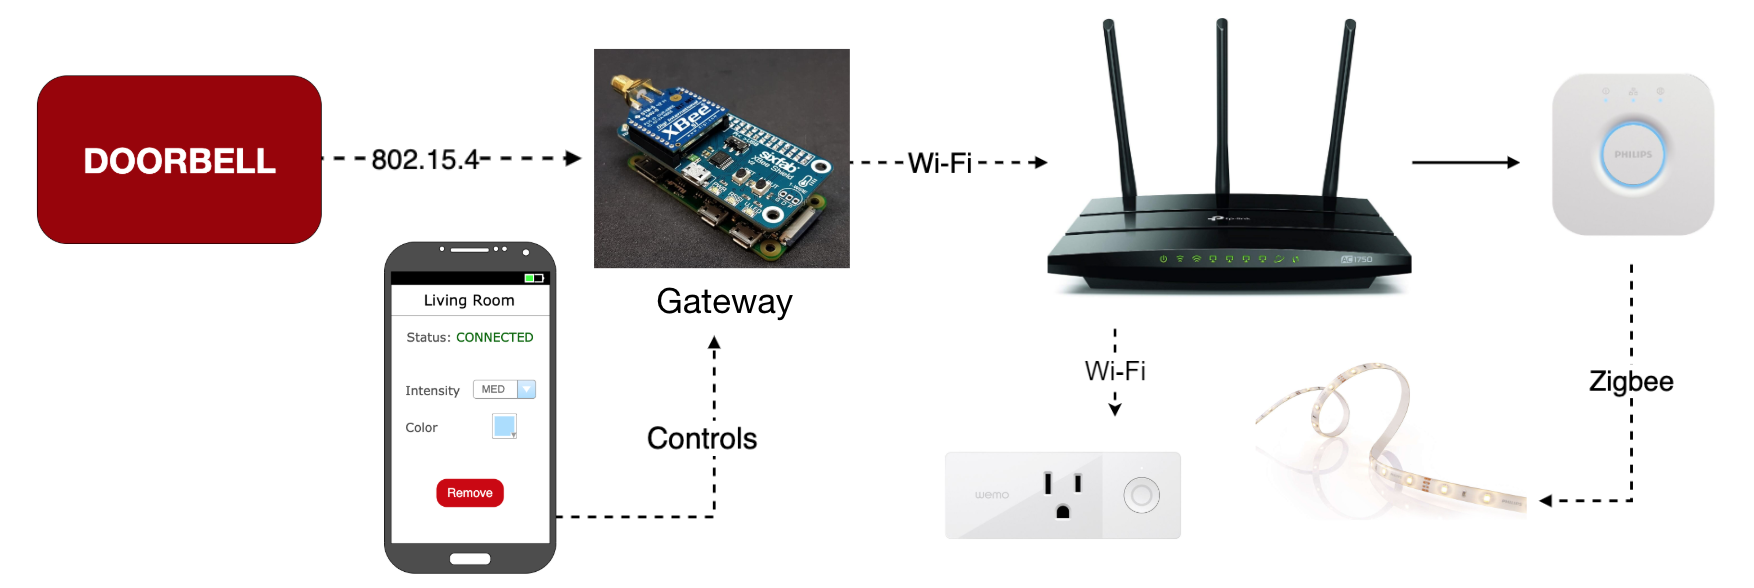
\includegraphics[width=0.8\textwidth]{senior-design-model.png}
  \centering
  \caption{Conceptual Model}
  \label{fig:conceptualmodel}
\end{figure}